\chptr{Descrizione del moto}
\marginpar{\minitoc}

\section{Moto del punto materiale}

\section{Il piano spazio-tempo}

\section{Moto in una dimensione}
\subsection{Moto rettilineo uniforme}
\subsection{Moto rettilineo uniformemente accelerato}

\section{Altri moti}
\subsection{Moto in più dimensioni}
\subsection{Moto circolare uniforme}
\subsection{Moto armonico semplice}


\section*{Moto del punto}
Un corpo è in moto quando la sua posizione cambia nel tempo. Nel descrivere il
moto, si introdurrà la seguente semplificazione: Gli oggetti saranno
trattati come \textit{punti materiali}, ovvero concentrati in un punto
adimensionale. In particolare, \textit{le dimensioni dell'oggetto del quale si
intende studiare il moto saranno considerate trascurabili rispetto a quelle
dell'ambiente circostante}.

Come comportarsi in situazioni come la descrizione del moto di un'auto, che è
un corpo \textit{esteso}? In questo corso, possiamo supporre che tutta l'auto
si concentri in un punto specifico, o che venga trattato il moto di una sua
parte puntiforme: Un pezzo del lunotto, lo specchietto retrovisore, la punta del
paraurti anteriore o una parte molto piccola rispetto a tutto il resto. È tuttavia fondamentale che, se si
parla del moto dell'auto, si intenda sempre quel punto che abbiamo scelto in partenza.

\subsection*{Sistemi di riferimento}
Abbiamo detto che il moto è caratterizzato da un cambiamento di posizione. Il primo
passo nella descrizione del moto di un corpo consiste quindi nello stabilire il
modello da adottare per catturare il concetto di \textbf{posizione}. Sappiamo già
che i modelli della fisica si basano sul linguaggio matematico; il modello più
naturale che si possa adottare è dunque un sistema di assi cartesiani. Da qui, la
posizione del corpo può essere specificata mediante coordinate. Una speciale
coordinata è il tempo (in caso di moti in più di una dimensione spaziale, il
tempo viene spesso omesso dalla rappresentazione grafica).

\begin{marginfigure}
    \centering
    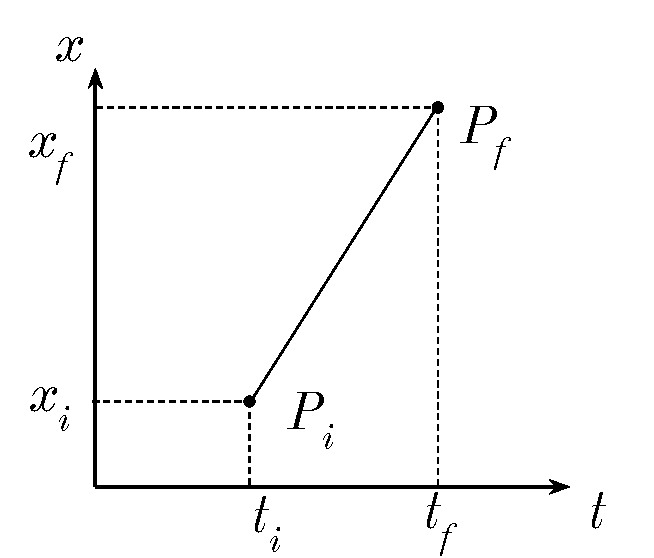
\includegraphics[width = \marginparwidth]{punto_sul_cartesiano.pdf}
    \caption{Sistema di riferimento con una sola dimensione spaziale ($x$)
    in funzione del tempo ($t$). All'istante $t_i$, il punto materiale $P$
    si trova nella posizione $x_i$}
    \label{point}
\end{marginfigure}

La scelta del sistema di riferimento di assi cartesiani è del tutto arbitraria\footnote{
Gli assi possono addirittura non essere ortogonali, purché si segua la \textit{regola del
parallelogramma} e si rinunci alle proprietà e alle regolarità matematiche degli
assi ortogonali, come il teorema di Pitagora per il calcolo del modulo dei
vettori.}, ma una volta fissata è necessario essere coerenti con essa.
Questo permette di riflettere sul fatto che il moto è sempre relativo al sitema di
riferimento adottato: cambiando sistema di riferimento, il moto cambia.

Fissando gli assi cartesiani, si fissa una componente di un \textit{sistema di
riferimento}. Intuitivamente, un sistema di riferimento è il ``punto di vista''
da cui si sceglie di effettuare misure ed osservazioni riguardo ad un certo
fenomeno.

\subsection*{Posizione e traiettoria}
Alla base della descrizione del moto, è importante individuare quelli che sono
chiamati \textit{posizione} e \textit{traiettoria}. Avendo assunto la semplificazione
del punto materiale, è intuibile che la posizione verrà descritta matematicamente
come una tupla di coordinate inserite in un sistema di assi cartesiani. Tra le
coordinate, è importante tenere presente anche il tempo. Di fatto, abbiamo
introdotto il moto definendolo come variazione della posizione nel tempo.

La traiettoria non è altro che la linea che unisce le posizioni occupate
successivamente dal corpo. Tratteremo prima moti con traiettorie rettilinee,
per poi passare a traiettorie curvilinee semplici, come il moto circolare.

\begin{tcolorbox}[colback = yellow!30, colframe = yellow!30!black, title = {Posizione e traiettoria}]
\begin{itemize}
    \item La posizione di un corpo è il punto nel quale esso si trova entro un
    determinato sistema di riferimento.

    \item La traiettoria di un corpo è l'insieme di posizioni occupate da esso
    durante il suo moto.
\end{itemize}
\end{tcolorbox}

\subsection*{Distanza e spostamento}
Durante il moto, è possibile registrare la \textbf{distanza} percorsa
dall'oggetto e il suo \textbf{spostamento}. Il primo è una grandezza
scalare e corrisponde alla distanza totale percorsa durante il tragitto
effettuato dall'oggetto in moto. Il secondo è una grandezza vettoriale e
corrisponde al cambiamento di posizione,
cioè la differenza tra la posizione iniziale e quella finale dell'oggetto:
\[ \Delta \mathbf{x} = \mathbf{x}_f - \mathbf{x}_i \]

\section*{Interpretazioni geometriche}

\begin{marginfigure}
    \centering
    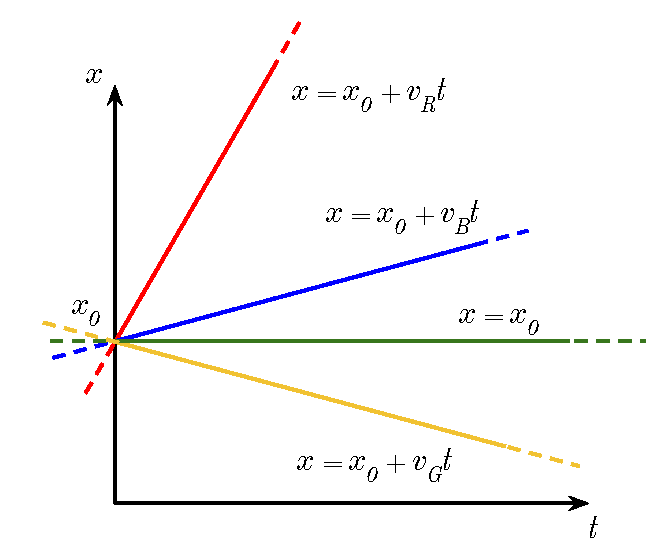
\includegraphics[width = \marginparwidth]{velocita_come_pendenza.pdf}
    \caption{Oggetti in moto rettilineo uniforme con velocità differenti}
\end{marginfigure}

\section*{Moto rettilineo uniforme}
\section*{Accelerazione}



\section*{Moto circolare}
Cambiamo ora la traiettoria dell'oggetto in moto, considerando quella circolare.
Per descrivere un moto circolare è conveniente impiegare coordinate differenti,
dette polari. Fissando il centro di un piano cartesiano al centro di una
circonferenza di raggio $r$, possiamo identificare la posizione di ogni punto
della circonferenza con la coppia $(r, \theta)$, dove $\theta$ è l'angolo
formato dalla semiretta appartenente al sistema di riferimento e dalla semiretta
che interseca la circonferenza nel punto desiderato (entrambe le semirette
hanno origine nel centro del piano cartesiano, quindi della circonferenza).

\begin{marginfigure}
    \centering
    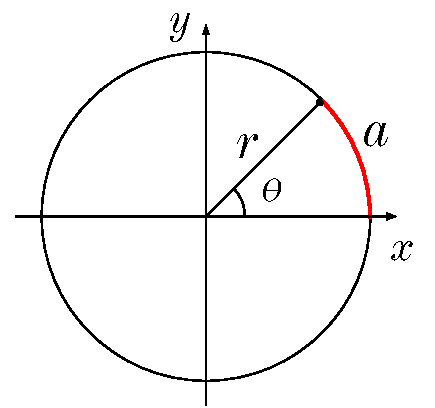
\includegraphics[width = \marginparwidth]{moto_circolare.pdf}
    \caption{Sistema di riferimento per un moto circolare.}
    \label{circref}
\end{marginfigure}

Assumeremo qui che $r$ non varia durante il moto. Per questo, viene omessa
la coordinata $r$ e si considera invece la posizione derivante da $\theta$,
detta anche \textit{posizione angolare}. Convenzionalmente, $\theta > 0$ se
misurato in senso antiorario a partire dall'asse di riferimento (come in
Figura \ref{circref}). Si utilizzano inoltre i \textit{radianti} per misurare
$\theta$. I radianti tornano infatti comodi, perché permettono di semplificare
le relazioni tra le grandezze in gioco durante il moto circolare. Innanzitutto,
dato l'arco $a$ in Figura \ref{circref}, vale la relazione \[ a = r\theta \]
Di fatto, la lunghezza totale della circonferenza corrisponde a $C = 2\pi r$,
dove $2\pi$ corrisponde ad un angolo giro espresso in radianti.

\subsection*{Velocità angolare e velocità tangenziale}
Studiamo ora il cambiamento della posizione angolare nel tempo. Come per il
moto rettilineo, possiamo considerare il rapporto tra lo spostamento angolare
e l'intervallo di tempo trascorso. Da qui, si ottiene la velocità angolare:
\[ \omega = \frac{d\theta}{dt} \]
In ogni istante, una particella in moto circolare si muove in direzione
tangenziale alla traiettoria.
\begin{marginfigure}
    \centering
    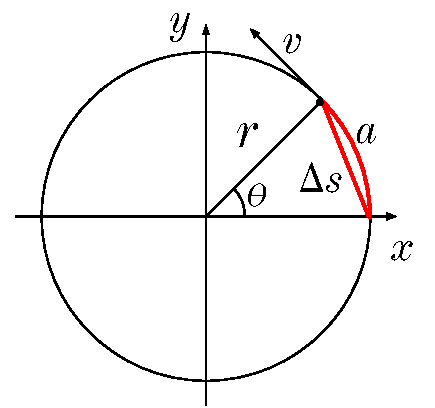
\includegraphics[width = \marginparwidth]{velocita_tangenziale.pdf}
    \caption{Velocità tangenziale.}
    \label{circspeed}
\end{marginfigure}
È chiaro che la particella, muovendosi, copre una certa distanza sulla
circonferenza in un dato intervallo di tempo. Possiamo quindi affermare
che essa ha una velocità, detta \textit{tangenziale}, $v$, oltre che
quella angolare $\omega$. Cerciamo una relazione tra esse: supponiamo che
la particella effettui, in un intervallo infinitesimo $\Delta t$, uno
spostamento angolare altrettanto piccolo $\Delta\theta$ come mostrato in
Figura \ref{circspeed}. Lo spostamento $\Delta s$, dato dalla corda che
sottende l'angolo $\Delta\theta$, approssima l'arco $a = r\Delta\theta$. Quindi:
\[ v = \lim_{\Delta t \to 0}\frac{\Delta s}{\Delta t} = \lim_{\Delta t \to 0} \frac{r\Delta\theta}{\Delta t} = r\lim_{\Delta t \to 0}\frac{\Delta\theta}{\Delta t} = r\omega \]
Abbiamo quindi ottenuto la relazione cercata:
\[ v = r\omega \]
Notare come $v\propto r$, al contrario di $\omega$. Ciò significa che,
assumendo una velocità angolare costante, la velocità tangenziale è tanto
maggiore quanto più $r$ cresce.

\subsection*{Moto circolare uniforme}
Un moto circolare uniforme è un moto circolare con velocità \textit{angolare} costante.
Le regolarità di questo tipo di moto permettono di studiare altre grandezze
importanti per il moto circolare: periodi e accelerazioni.

\subsubsection*{Periodo e frequenza}
La particolarità di questo moto è la sua periodicità, perché esso si ripete
ciclicamente nel tempo. In particolare, un oggetto torna ad occupare la medesima
posizione iniziale dopo un certo intervallo di tempo, chiamato \textbf{periodo} ($T$):
in altre parole, il tempo necessario per compiere ``un giro (ciclo) completo''.
Nel nostro caso, un giro completo corrisponde all'intera circonferenza $C = 2\pi$.
Sapendo che $\omega = \frac{d\theta}{dt}$, è immediato ricavare il periodo:
\[ T = \frac{2\pi}{\omega} \]
Si impiega spesso anche la \textbf{frequenza}, che corrisponde al reciproco
del periodo:
\[ f = \frac{1}{T} \]
L'unità di misura è l'\textit{Hertz} (Hz), ovvero ``cicli al secondo'' (s$^{-1}$),
quindi il numero di cicli compiuti nell'unità di tempo.

\subsubsection*{Accelerazione centripeta}
Riprendendo la prima legge della dinamica, sappiamo che un corpo permane nel
suo stato di moto rettilineo uniforme a meno dell'intervento di agenti esterni.
Nel caso dell'intervento di tali agenti, si osserva un'accelerazione
dell'oggetto, ovvero un cambiamento del suo stato di moto e dunque della sua
velocità. Non viene specificato se questo cambiamento avviene al \textit{modulo}
oppure alla \textit{direzione} della velocità. Infatti, la velocità è una
grandezza vettoriale e una variazione di anche una sola delle sue caratteristiche
comporta un'accelerazione. Per questo motivo, nonostante il modulo della velocità
tangenziale di un corpo in moto circolare uniforme sia costante, la direzione
del suo vettore cambia.

Vi è però il problema aperto di trovare l'agente esterno (la forza) che
mantiene l'oggetto (dotato di massa) nella traiettoria del suo moto circolare.
Esso può essere di varia natura: la tensione di una corda attaccata ad una
pallina che viene fatta roteare; la forza di gravitazione universale che
mantiene in orbita (assumiamo circolare) un pianeta intorno ad un sole; la forza
elettrica che mantiene un elettrone vicino al nucleo (secondo un modello classico
dell'atomo).

Vista quindi l'esistenza di un'accelerazione determinata da un agente esterno,
rimane da capire come è fatto il suo vettore (modulo, verso e direzione).
L'esperienza ci dice che questa accelerazione: (1) cresce con l'aumentare della
velocità angolare; (2) è diretta verso il centro della circonferenza. Ma come
dimostrarlo formalmente per tutti i moti circolari uniformi? Consideriamo la
situazione in Figura \ref{circolare}.
\begin{marginfigure}
    \centering
    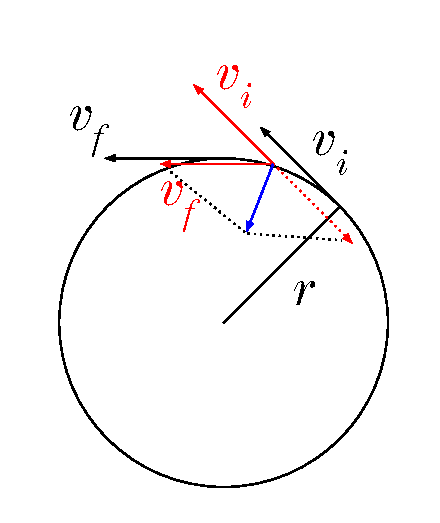
\includegraphics[width = \marginparwidth]{accelerazione_centripeta.pdf}
    \caption{Dimostrazione delle caratteristiche geometriche del vettore accelerazione centripeta.}
    \label{circolare}
\end{marginfigure}
consideriamo una variazione molto piccola nella posizione angolare dell'oggetto,
che parte con una velocità iniziale $\mathbf{v}_i$ e termina con la
velocità finale $\mathbf{v}_f$, uguali in modulo ma diverse in direzione.
Come già detto, possiamo esprimere l'accelerazione come variazione della
velocità tangenziale.

\[ \mathbf{a} = \frac{d\mathbf{v}}{dt} \simeq \frac{\Delta\mathbf{v}}{\Delta t} \]

\noindent Concentriamoci sul termine $\Delta\mathbf{v}$.

\[ \Delta\mathbf{v} = \mathbf{v}_f - \mathbf{v}_i = \mathbf{v}_f + (-\mathbf{v}_i) \]
Geometricamente, i vettori velocità si sommano secondo la ``regola del parallelogramma''
come mostrato nella Figura. Con i dovuti formalismi geometrici, sapendo che il
modulo di $v$ è sempre costante, possiamo dimostrare che l'accelerazione è
effettivamente centripeta e ortogonale alla velocità tangenziale, ovvero il
suo vettore punta sempre verso il centro della circonferenza. Sempre dalla Figura,
possiamo osservare che al crescere di $v$ cresce anche $a$; tenendo poi
presente che la variazione $\Delta \mathbf{v}$, che è un vettore,
viene moltiplicata per la quantità scalare $\frac{1}{\Delta t}$, il vettore
risultante dell'accelerazione cresce in modulo quanto più piccolo diventa
l'intervallo $\Delta t$: ovvero la velocità dell'oggetto è maggiore.
Dimostreremo più
avanti che la relazione precisa tra i moduli di queste grandezze è data da
\[ a = \frac{v^2}{r} = \omega^2 r \]

\section*{Moto armonico}
Supponiamo di osservare un oggetto in moto circolare uniforme, ma invece di
vederlo ``dall'alto'' lo guardiamo con la riconferenza della traiettoria
posta orizzontalmente. Da questo punto di vista, vedremo l'oggetto \textit{oscillare}
a destra e sinistra all'interno di uno spazio la cui larghezza corrisponde al
diametro della circonferenza. Ciò che si vede è un moto particolare, il
\textit{moto armonico semplice}.

Dalla Figura \ref{armonicosemplice} possiamo notare che, fissato il solito
sistema di riferimento $xy$, il moto armonico semplice non è altro che la
proiezione sugli assi di un moto circolare uniforme. Per questo motivo,
possiamo descrivere la posizione dell'oggetto caratterizzato da tale moto:
\begin{marginfigure}
    \centering
    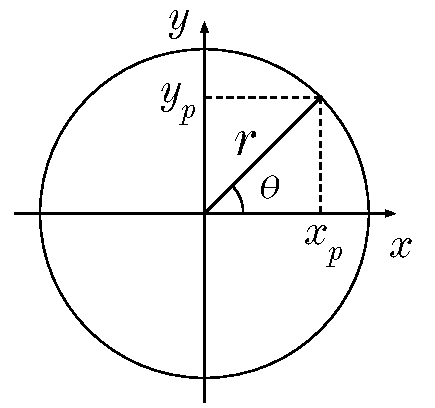
\includegraphics[width = \marginparwidth]{da_circolare_ad_armonico.pdf}
    \caption{Modello di moti armonici semplici a partire da proiezioni
    di un moto circolare uniforme.}
    \label{armonicosemplice}
\end{marginfigure}
\[
    \begin{cases}
        x_p(t) = r\cos\theta = r\cos(\omega t)\\
        y_p(t) = r\sin\theta = r\sin(\omega t)
    \end{cases}
\]
Possiamo quindi notare che il moto circolare è la composizione di due moti
armonici.
Sapendo che la velocità corrisponde alla derivata della funzione che
descrive la posizione:
\[
    \begin{cases}
        v_x(t) = -\omega R \sin(\omega t)\\
        v_y(t) = \omega R \cos(\omega t)
    \end{cases}
\]
Derivando nuovamente, otteniamo l'accelerazione:
\[
    \begin{cases}
        a_x(t) = -\omega^2 R\cos(\omega t)\\
        a_y(t) = -\omega^2 R\sin(\omega t)
    \end{cases}
\]
Esiste anche una dimostrazione geometrica di tali relazioni, che non impiega
esplicitamente i metodi del calcolo infinitesimale. È sufficiente tenere in
considerazione la posizione angolare $\theta$, avere dimestichezza con le
funzioni sinusoidali e ricordare direzione e verso dei vettori velocità
tangenziale e accelerazione centripeta durante un moto circolare uniforme.

\subsubsection*{Relazione tra accelerazione centripeta e velocità}
Siamo ora in grado di mostrare l'origine della relazione $a = \frac{v^2}{r} = \omega^2 r$
tra accelerazione centripeta e velocità (angolare e tangenziale) in un moto
circolare uniforme.

Osserviamo che il sistema che descrive l'accelerazione del moto armonico
contiene i termini $r\cos(\omega t)$ e $r\sin(\omega t)$: le coordinate del
punto in moto circolare uniforme in funzione del tempo. Dunque

\[
    \begin{cases}
        a_x(t) = -\omega^2 r\cos(\omega t)\\
        a_y(t) = -\omega^2 r\sin(\omega t)
    \end{cases}
    \Rightarrow
    \begin{cases}
        a_x(t) = -\omega^2 x(t)\\
        a_y(t) = -\omega^2 y(t)
    \end{cases}
\]
Queste non sono altro che le componenti dell'accelerazione centripeta
solidali al sistema di riferimento di assi $xy$. Sapendo che il modulo
di un vettore corrisponde a $|\mathbf{r}| = r = \sqrt{x_r^2 + y_r^2}$
(con $x_r,y_r$ le componenti del vettore $r$ rispetto ad un sistema di
assi ortogonali $xy$), è immediato mostrare che
\[ |\mathbf{a}| = a = \sqrt{(-\omega^2 x)^2 + (-\omega^2 y)^2} = \sqrt{\omega^4x^2 + \omega^4y^2} = \omega^2 \sqrt{x^2 + y^2} = \omega^2 r \]

Dal precedente sistema, è possibile capire perché il vettore dell'accelerazione
è diretto verso il centro della circonferenza: $x$ ed $y$ sono le componenti
del \textit{vettore posizione} dell'oggetto in movimento; tale vettore
non è altro che una freccia di modulo uguale alla lunghezza del raggio e la
cui punta indica il punto in cui il corpo si trova sulla circonferenza,
dunque questo vettore punta verso l'esterno; ma dato che ogni componente
viene moltiplicata per la quantità negativa $-\omega^2$, il vettore
accelerazione centripeta non può che puntare nel verso opposto, quindi
verso il centro della circonferenza. L'equazione vettoriale è dunque la
seguente:
\[ \mathbf{a} = -\frac{\mathbf{v}^2}{\mathbf{r}} \]

\section*{Moto nel piano}

\subsubsection*{Parabola di un proiettile}
\[
    \begin{cases}
        x = v_{0,x}t\\
        y = v_{0,y}t - \frac{1}{2}t^2
    \end{cases}
\]
Esprimiamo $y$ in funzione di $x$:
\[
    y = \frac{v_{0,y}}{v_{0,x}}x - \frac{1}{2}\frac{g}{v_{0,x}^2}x^2 = Bx - Cx^2
\]
Tangente a questa parabola:
\[
    y' = B - 2Cx
\]

\subsection*{Vettori}
Vettori posizione e spostamento.
\[ \Delta\mathbf{s} = \mathbf{s}_f - \mathbf{s}_i \]

Vettore velocità
\[ \mathbf{v} = \lim_{\Delta t \to 0}\frac{\Delta\mathbf{s}}{\Delta t} = \frac{d\mathbf{s}}{dt} \sim ds\cdot\frac{1}{dt} \]
Per definizione \textit{sempre} tangente alla traiettoria. La traiettoria
è la serie dei punti che si ottiene percorrendo per tratti infinitesimi le
velocità istantanee.

Accelerazione tangente e accelerazione normale.


\subsubsection*{Esercizio}
$|\mathbf{v}_i| = 50\text{ km/h}$, $|\mathbf{v}_f| = 100\text{ km/h}$,
$m = 1800\text{ kg}$, $R = 20\text{ m}$, $\Delta t = 2\text{ s}$. $|\mathbf{F}_n| = ?$ (forza normale),
$|\mathbf{a}_t| = ?$. Assumiamo che l'auto acceleri con costanza tra le
due velocità.

\begin{itemize}
    \item $a_{n,i} = \frac{v_i^2}{R}$, $a_{n,f} = \frac{v_f^2}{R}$
    \item $F_{n,i} = ma_{n,i} \simeq 17100 \text{ N}$, $F_{n,f} = ma_{n,f} \simeq 68400\text{ N}$
    \item $|\mathbf{a}_t| = \textit{cost} = \frac{|\Delta\mathbf{v}|}{\Delta t} \simeq 6,95\text{ m/s}^2$
\end{itemize}

\section*{Recap}
\[ \mathbf{x} = \mathbf{x_0} + \mathbf{v}(t - t_0) \]
Semplificazioni in termini di variazioni, infinità.